\documentclass[]{article}
\usepackage{lmodern}
\usepackage{amssymb,amsmath}
\usepackage{ifxetex,ifluatex}
\usepackage{fixltx2e} % provides \textsubscript
\ifnum 0\ifxetex 1\fi\ifluatex 1\fi=0 % if pdftex
  \usepackage[T1]{fontenc}
  \usepackage[utf8]{inputenc}
\else % if luatex or xelatex
  \ifxetex
    \usepackage{mathspec}
  \else
    \usepackage{fontspec}
  \fi
  \defaultfontfeatures{Ligatures=TeX,Scale=MatchLowercase}
\fi
% use upquote if available, for straight quotes in verbatim environments
\IfFileExists{upquote.sty}{\usepackage{upquote}}{}
% use microtype if available
\IfFileExists{microtype.sty}{%
\usepackage[]{microtype}
\UseMicrotypeSet[protrusion]{basicmath} % disable protrusion for tt fonts
}{}
\PassOptionsToPackage{hyphens}{url} % url is loaded by hyperref
\usepackage[unicode=true]{hyperref}
\hypersetup{
            pdftitle={Project 2: Modeling, Testing, and Predicting},
            pdfauthor={Shannon Owings},
            pdfborder={0 0 0},
            breaklinks=true}
\urlstyle{same}  % don't use monospace font for urls
\usepackage[margin=1in]{geometry}
\usepackage{color}
\usepackage{fancyvrb}
\newcommand{\VerbBar}{|}
\newcommand{\VERB}{\Verb[commandchars=\\\{\}]}
\DefineVerbatimEnvironment{Highlighting}{Verbatim}{commandchars=\\\{\}}
% Add ',fontsize=\small' for more characters per line
\usepackage{framed}
\definecolor{shadecolor}{RGB}{248,248,248}
\newenvironment{Shaded}{\begin{snugshade}}{\end{snugshade}}
\newcommand{\KeywordTok}[1]{\textcolor[rgb]{0.13,0.29,0.53}{\textbf{#1}}}
\newcommand{\DataTypeTok}[1]{\textcolor[rgb]{0.13,0.29,0.53}{#1}}
\newcommand{\DecValTok}[1]{\textcolor[rgb]{0.00,0.00,0.81}{#1}}
\newcommand{\BaseNTok}[1]{\textcolor[rgb]{0.00,0.00,0.81}{#1}}
\newcommand{\FloatTok}[1]{\textcolor[rgb]{0.00,0.00,0.81}{#1}}
\newcommand{\ConstantTok}[1]{\textcolor[rgb]{0.00,0.00,0.00}{#1}}
\newcommand{\CharTok}[1]{\textcolor[rgb]{0.31,0.60,0.02}{#1}}
\newcommand{\SpecialCharTok}[1]{\textcolor[rgb]{0.00,0.00,0.00}{#1}}
\newcommand{\StringTok}[1]{\textcolor[rgb]{0.31,0.60,0.02}{#1}}
\newcommand{\VerbatimStringTok}[1]{\textcolor[rgb]{0.31,0.60,0.02}{#1}}
\newcommand{\SpecialStringTok}[1]{\textcolor[rgb]{0.31,0.60,0.02}{#1}}
\newcommand{\ImportTok}[1]{#1}
\newcommand{\CommentTok}[1]{\textcolor[rgb]{0.56,0.35,0.01}{\textit{#1}}}
\newcommand{\DocumentationTok}[1]{\textcolor[rgb]{0.56,0.35,0.01}{\textbf{\textit{#1}}}}
\newcommand{\AnnotationTok}[1]{\textcolor[rgb]{0.56,0.35,0.01}{\textbf{\textit{#1}}}}
\newcommand{\CommentVarTok}[1]{\textcolor[rgb]{0.56,0.35,0.01}{\textbf{\textit{#1}}}}
\newcommand{\OtherTok}[1]{\textcolor[rgb]{0.56,0.35,0.01}{#1}}
\newcommand{\FunctionTok}[1]{\textcolor[rgb]{0.00,0.00,0.00}{#1}}
\newcommand{\VariableTok}[1]{\textcolor[rgb]{0.00,0.00,0.00}{#1}}
\newcommand{\ControlFlowTok}[1]{\textcolor[rgb]{0.13,0.29,0.53}{\textbf{#1}}}
\newcommand{\OperatorTok}[1]{\textcolor[rgb]{0.81,0.36,0.00}{\textbf{#1}}}
\newcommand{\BuiltInTok}[1]{#1}
\newcommand{\ExtensionTok}[1]{#1}
\newcommand{\PreprocessorTok}[1]{\textcolor[rgb]{0.56,0.35,0.01}{\textit{#1}}}
\newcommand{\AttributeTok}[1]{\textcolor[rgb]{0.77,0.63,0.00}{#1}}
\newcommand{\RegionMarkerTok}[1]{#1}
\newcommand{\InformationTok}[1]{\textcolor[rgb]{0.56,0.35,0.01}{\textbf{\textit{#1}}}}
\newcommand{\WarningTok}[1]{\textcolor[rgb]{0.56,0.35,0.01}{\textbf{\textit{#1}}}}
\newcommand{\AlertTok}[1]{\textcolor[rgb]{0.94,0.16,0.16}{#1}}
\newcommand{\ErrorTok}[1]{\textcolor[rgb]{0.64,0.00,0.00}{\textbf{#1}}}
\newcommand{\NormalTok}[1]{#1}
\usepackage{graphicx,grffile}
\makeatletter
\def\maxwidth{\ifdim\Gin@nat@width>\linewidth\linewidth\else\Gin@nat@width\fi}
\def\maxheight{\ifdim\Gin@nat@height>\textheight\textheight\else\Gin@nat@height\fi}
\makeatother
% Scale images if necessary, so that they will not overflow the page
% margins by default, and it is still possible to overwrite the defaults
% using explicit options in \includegraphics[width, height, ...]{}
\setkeys{Gin}{width=\maxwidth,height=\maxheight,keepaspectratio}
\IfFileExists{parskip.sty}{%
\usepackage{parskip}
}{% else
\setlength{\parindent}{0pt}
\setlength{\parskip}{6pt plus 2pt minus 1pt}
}
\setlength{\emergencystretch}{3em}  % prevent overfull lines
\providecommand{\tightlist}{%
  \setlength{\itemsep}{0pt}\setlength{\parskip}{0pt}}
\setcounter{secnumdepth}{0}
% Redefines (sub)paragraphs to behave more like sections
\ifx\paragraph\undefined\else
\let\oldparagraph\paragraph
\renewcommand{\paragraph}[1]{\oldparagraph{#1}\mbox{}}
\fi
\ifx\subparagraph\undefined\else
\let\oldsubparagraph\subparagraph
\renewcommand{\subparagraph}[1]{\oldsubparagraph{#1}\mbox{}}
\fi

% set default figure placement to htbp
\makeatletter
\def\fps@figure{htbp}
\makeatother


\title{Project 2: Modeling, Testing, and Predicting}
\author{Shannon Owings}
\date{4/22/2020}

\begin{document}
\maketitle

\subsection{0. Introduction}\label{introduction}

My dataset for Project 2 is entitled ``Automobile'' and has 6 variables:
fuel-type, body-style, num-of-cylinders, engine-size, city-mpg, and
highway-mpg. Three of these variables are categorical and three are
numeric. The categorical variables are the fuel type of the car (gas or
diesel), body style of the car (convertible, hatchback, etc.), and
number of cylinders (four, five, six, etc.). The numeric variables are
engine size, city miles per gallon, highway miles per gallon, and price.
These variables provide information on 199 different observations. This
data was found at Kaggle.com, which pulled its information from 1985
Ward's Automotice Yearbook. I chose this dataset because my father is a
mechanic and I've always wanted to learn about cars, so this a great way
to start!

\subsection{1. MANOVA testing}\label{manova-testing}

\begin{Shaded}
\begin{Highlighting}[]
\KeywordTok{library}\NormalTok{(tidyverse)}
\KeywordTok{library}\NormalTok{(readr)}
\NormalTok{Automobile <-}\StringTok{ }\KeywordTok{read_csv}\NormalTok{(}\StringTok{"/stor/home/smo884/Project 2/Project2data.csv"}\NormalTok{)}
\NormalTok{Automobile <-}\StringTok{ }\NormalTok{Automobile }\OperatorTok\StringTok{ }\KeywordTok{rename}\NormalTok{(}\DataTypeTok{highway.mpg =} \StringTok{`}\DataTypeTok{highway-mpg}\StringTok{`}\NormalTok{, }
    \DataTypeTok{body.style =} \StringTok{`}\DataTypeTok{body-style}\StringTok{`}\NormalTok{, }\DataTypeTok{fuel.type =} \StringTok{`}\DataTypeTok{fuel-type}\StringTok{`}\NormalTok{, }\DataTypeTok{num.of.cylinders =} \StringTok{`}\DataTypeTok{num-of-cylinders}\StringTok{`}\NormalTok{, }
    \DataTypeTok{engine.size =} \StringTok{`}\DataTypeTok{engine-size}\StringTok{`}\NormalTok{, }\DataTypeTok{city.mpg =} \StringTok{`}\DataTypeTok{city-mpg}\StringTok{`}\NormalTok{)}

\CommentTok{# Multivariate Plots}
\KeywordTok{library}\NormalTok{(ggplot2)}
\KeywordTok{ggplot}\NormalTok{(Automobile, }\KeywordTok{aes}\NormalTok{(}\DataTypeTok{x =}\NormalTok{ engine.size, }\DataTypeTok{y =}\NormalTok{ city.mpg }\OperatorTok{+}\StringTok{ }\NormalTok{highway.mpg)) }\OperatorTok{+}\StringTok{ }
\StringTok{    }\KeywordTok{geom_point}\NormalTok{(}\DataTypeTok{alpha =} \FloatTok{0.5}\NormalTok{) }\OperatorTok{+}\StringTok{ }\KeywordTok{geom_density_2d}\NormalTok{(}\DataTypeTok{h =} \DecValTok{2}\NormalTok{) }\OperatorTok{+}\StringTok{ }\KeywordTok{coord_fixed}\NormalTok{() }\OperatorTok{+}\StringTok{ }
\StringTok{    }\KeywordTok{facet_wrap}\NormalTok{(}\OperatorTok{~}\NormalTok{body.style)}
\end{Highlighting}
\end{Shaded}

\begin{center}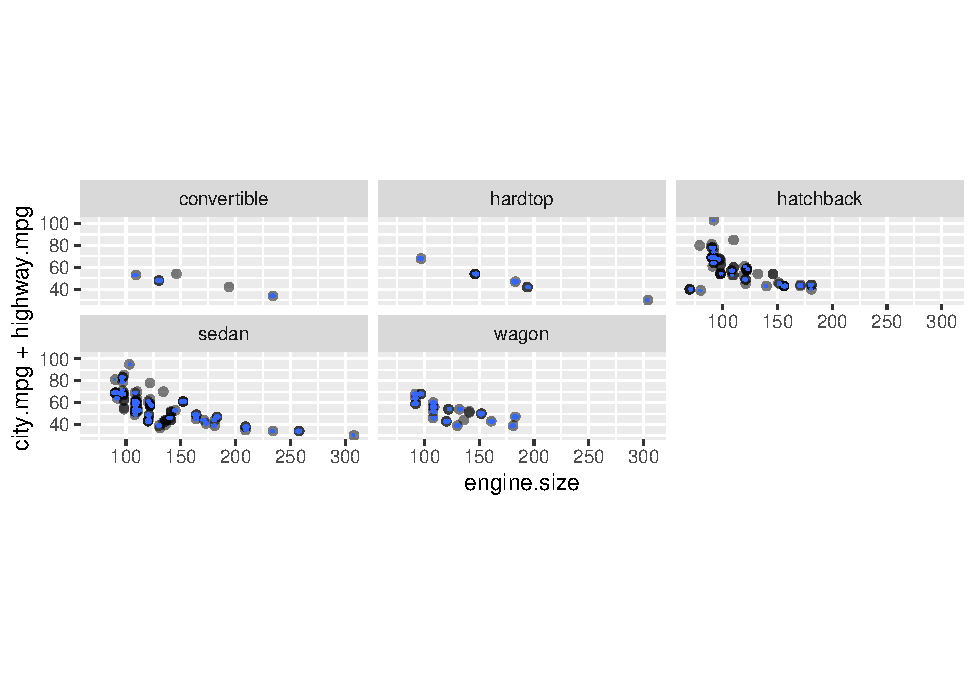
\includegraphics{project2_files/figure-latex/unnamed-chunk-1-1} \end{center}

\begin{Shaded}
\begin{Highlighting}[]
\KeywordTok{ggplot}\NormalTok{(Automobile, }\KeywordTok{aes}\NormalTok{(}\DataTypeTok{x =}\NormalTok{ city.mpg, }\DataTypeTok{y =}\NormalTok{ highway.mpg)) }\OperatorTok{+}\StringTok{ }\KeywordTok{geom_point}\NormalTok{(}\DataTypeTok{alpha =} \FloatTok{0.5}\NormalTok{) }\OperatorTok{+}\StringTok{ }
\StringTok{    }\KeywordTok{geom_density_2d}\NormalTok{(}\DataTypeTok{h =} \DecValTok{2}\NormalTok{) }\OperatorTok{+}\StringTok{ }\KeywordTok{coord_fixed}\NormalTok{() }\OperatorTok{+}\StringTok{ }\KeywordTok{facet_wrap}\NormalTok{(}\OperatorTok{~}\NormalTok{body.style)}
\end{Highlighting}
\end{Shaded}

\begin{center}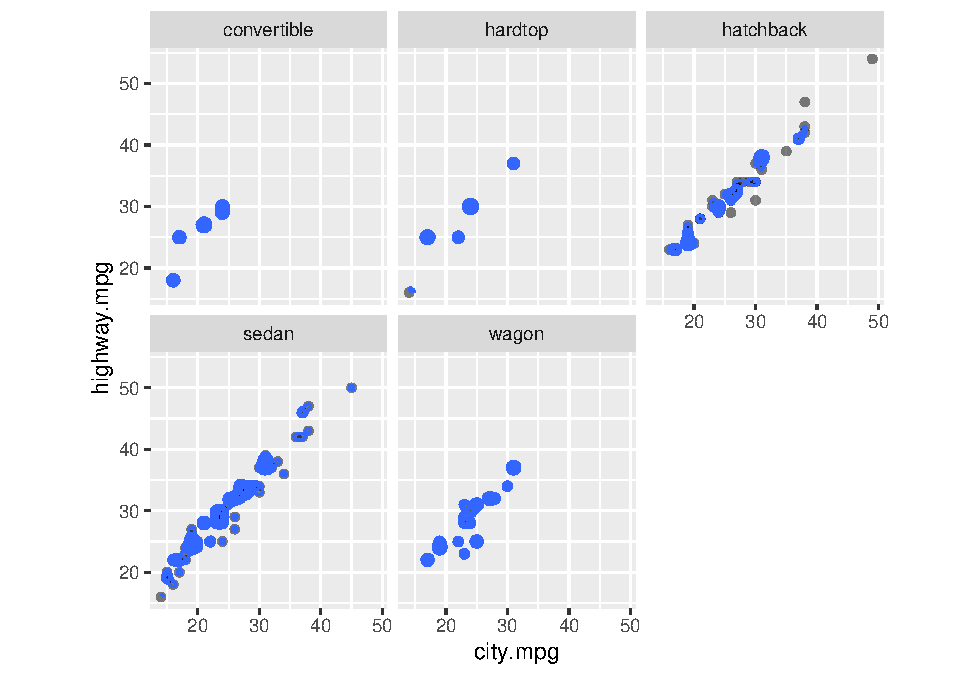
\includegraphics{project2_files/figure-latex/unnamed-chunk-1-2} \end{center}

\begin{Shaded}
\begin{Highlighting}[]
\CommentTok{# Homogeneity of covariances}
\KeywordTok{library}\NormalTok{(dplyr)}
\NormalTok{covmats <-}\StringTok{ }\NormalTok{Automobile }\OperatorTok\StringTok{ }\KeywordTok{group_by}\NormalTok{(body.style) }\OperatorTok\StringTok{ }\KeywordTok{do}\NormalTok{(}\DataTypeTok{covs =} \KeywordTok{cov}\NormalTok{(.[}\DecValTok{4}\OperatorTok{:}\DecValTok{6}\NormalTok{]))}
\ControlFlowTok{for}\NormalTok{ (i }\ControlFlowTok{in} \DecValTok{1}\OperatorTok{:}\DecValTok{5}\NormalTok{) \{}
    \KeywordTok{print}\NormalTok{(}\KeywordTok{as.character}\NormalTok{(covmats}\OperatorTok{$}\NormalTok{body.style[i]))}
    \KeywordTok{print}\NormalTok{(covmats}\OperatorTok{$}\NormalTok{covs[i])}
\NormalTok{\}}
\end{Highlighting}
\end{Shaded}

\begin{verbatim}
## [1] "convertible"
## [[1]]
##             engine.size city.mpg highway.mpg
## engine.size    2236.167   -141.9      -179.0
## city.mpg       -141.900     11.5        13.0
## highway.mpg    -179.000     13.0        18.4
## 
## [1] "hardtop"
## [[1]]
##             engine.size   city.mpg highway.mpg
## engine.size   3717.3571 -299.17857  -364.92857
## city.mpg      -299.1786   29.41071    30.96429
## highway.mpg   -364.9286   30.96429    37.07143
## 
## [1] "hatchback"
## [[1]]
##             engine.size   city.mpg highway.mpg
## engine.size    845.9344 -107.00814  -106.15355
## city.mpg      -107.0081   44.33379    43.02284
## highway.mpg   -106.1536   43.02284    43.46404
## 
## [1] "sedan"
## [[1]]
##             engine.size   city.mpg highway.mpg
## engine.size   1665.0248 -174.45909  -199.76461
## city.mpg      -174.4591   39.80318    42.56253
## highway.mpg   -199.7646   42.56253    47.83403
## 
## [1] "wagon"
## [[1]]
##             engine.size  city.mpg highway.mpg
## engine.size   722.14000 -74.24333   -90.46333
## city.mpg      -74.24333  17.79000    17.92833
## highway.mpg   -90.46333  17.92833    22.12667
\end{verbatim}

\begin{Shaded}
\begin{Highlighting}[]
\CommentTok{# MANOVA test}
\NormalTok{man1 <-}\StringTok{ }\KeywordTok{manova}\NormalTok{(}\KeywordTok{cbind}\NormalTok{(engine.size, city.mpg, highway.mpg) }\OperatorTok{~}\StringTok{ }\NormalTok{body.style, }
    \DataTypeTok{data =}\NormalTok{ Automobile)}
\KeywordTok{summary}\NormalTok{(man1)}
\end{Highlighting}
\end{Shaded}

\begin{verbatim}
##             Df Pillai approx F num Df den Df    Pr(>F)    
## body.style   4 0.2012   3.4867     12    582 5.397e-05 ***
## Residuals  194                                            
## ---
## Signif. codes:  0 '***' 0.001 '**' 0.01 '*' 0.05 '.' 0.1 ' ' 1
\end{verbatim}

\begin{Shaded}
\begin{Highlighting}[]
\KeywordTok{summary.aov}\NormalTok{(man1)}
\end{Highlighting}
\end{Shaded}

\begin{verbatim}
##  Response engine.size :
##              Df Sum Sq Mean Sq F value    Pr(>F)    
## body.style    4  37601  9400.2  6.9196 3.157e-05 ***
## Residuals   194 263548  1358.5                      
## ---
## Signif. codes:  0 '***' 0.001 '**' 0.01 '*' 0.05 '.' 0.1 ' ' 1
## 
##  Response city.mpg :
##              Df Sum Sq Mean Sq F value  Pr(>F)  
## body.style    4  348.3  87.086  2.3213 0.05826 .
## Residuals   194 7278.3  37.517                  
## ---
## Signif. codes:  0 '***' 0.001 '**' 0.01 '*' 0.05 '.' 0.1 ' ' 1
## 
##  Response highway.mpg :
##              Df Sum Sq Mean Sq F value  Pr(>F)  
## body.style    4  451.8  112.94  2.6878 0.03256 *
## Residuals   194 8151.9   42.02                  
## ---
## Signif. codes:  0 '***' 0.001 '**' 0.01 '*' 0.05 '.' 0.1 ' ' 1
\end{verbatim}

\begin{Shaded}
\begin{Highlighting}[]
\KeywordTok{pairwise.t.test}\NormalTok{(Automobile}\OperatorTok{$}\NormalTok{engine.size, Automobile}\OperatorTok{$}\NormalTok{body.style, }
    \DataTypeTok{p.adj =} \StringTok{"none"}\NormalTok{)}
\end{Highlighting}
\end{Shaded}

\begin{verbatim}
## 
##  Pairwise comparisons using t tests with pooled SD 
## 
## data:  Automobile$engine.size and Automobile$body.style 
## 
##           convertible hardtop hatchback sedan  
## hardtop   0.33890     -       -         -      
## hatchback 0.00611     9.8e-06 -         -      
## sedan     0.07738     0.00072 0.00744   -      
## wagon     0.04811     0.00058 0.23852   0.48855
## 
## P value adjustment method: none
\end{verbatim}

\begin{Shaded}
\begin{Highlighting}[]
\KeywordTok{pairwise.t.test}\NormalTok{(Automobile}\OperatorTok{$}\NormalTok{highway.mpg, Automobile}\OperatorTok{$}\NormalTok{body.style, }
    \DataTypeTok{p.adj =} \StringTok{"none"}\NormalTok{)}
\end{Highlighting}
\end{Shaded}

\begin{verbatim}
## 
##  Pairwise comparisons using t tests with pooled SD 
## 
## data:  Automobile$highway.mpg and Automobile$body.style 
## 
##           convertible hardtop hatchback sedan
## hardtop   0.721       -       -         -    
## hatchback 0.029       0.048   -         -    
## sedan     0.085       0.148   0.194     -    
## wagon     0.357       0.577   0.028     0.172
## 
## P value adjustment method: none
\end{verbatim}

\begin{Shaded}
\begin{Highlighting}[]
\CommentTok{# Type I Error}
\DecValTok{1} \OperatorTok{-}\StringTok{ }\FloatTok{0.95}\OperatorTok{^}\DecValTok{14}
\end{Highlighting}
\end{Shaded}

\begin{verbatim}
## [1] 0.512325
\end{verbatim}

Before performing a MANOVA test, I tested the data to make sure that it
met the MANOVA assumptions. These assumptions required that the dataset
include random samples and independent observations, multivariate
normality of DVs, homogeneity of within-group covariance matrices, and
no extreme univariate or multivariate outliers. The random sample
assumption was violated because the researcher found his data in 1985
Ward's Automotive Yearbook and did not conduct the random sampling
method. The independent observations assumption is met because the
occurrence of one observation does not provide any information about the
occurrence of another observation. For example, the price of one
automobile has no effect on the price of another automobile. The
multivariate normality assumption was tested by plotting the response
variables. Examination of bivariate density plots for each group
revealed deparures from multivariate normality and examination of
covariance matrices for each group revealed that the matrices were not
homogeneous. There also appeared to be a couple of multivariate
outliers, therefore it appears that most of the assumptions were
violated. Despite violation of these assumptions, MANOVA was considered
to be an appropriate analysis technique. I then performed a MANOVA test.
The result was significant, so I decided to run univariate ANOVAs to
determine exactly which are body type means are significant, or in other
words, which body type group means significantly differ. One-way ANOVAs
were performed for each response variable. The p-values for engine size
and highway mpg are significant, but the p-value for city mpg is not
significant. This means that for engine size and highway mpg, at least
one body style differs! To determine exactly which body styles differ, I
performed post hoc t-tests for the two ANOVAs that were significant. In
total I performed 14 hypothesis tests (1 MANOVA, 3 ANOVAs, and 10 post
hoc t-tests). The probability that I have made at least one type I error
is about 0.5123. The boneferroni adjusted significance level that I
should use is 0.00357 (0.05/14) and with this new significance level, I
determined which differences were significant between groups. The
hardtop is significantly different from the hatchback, sedan, and wagon
in terms of engine size. Before the bonferroni correction, none of the
post-hoc t-tests are significant for highway mpg.

\subsection{2. Randomization test}\label{randomization-test}

\begin{Shaded}
\begin{Highlighting}[]
\KeywordTok{library}\NormalTok{(tidyverse)}

\NormalTok{autorand <-}\StringTok{ }\KeywordTok{data.frame}\NormalTok{(}\DataTypeTok{hwympg =}\NormalTok{ Automobile}\OperatorTok{$}\NormalTok{highway.mpg, }\DataTypeTok{fueltype =}\NormalTok{ Automobile}\OperatorTok{$}\NormalTok{fuel.type)}

\KeywordTok{ggplot}\NormalTok{(autorand, }\KeywordTok{aes}\NormalTok{(hwympg, }\DataTypeTok{fill =}\NormalTok{ fueltype)) }\OperatorTok{+}\StringTok{ }\KeywordTok{geom_histogram}\NormalTok{(}\DataTypeTok{bins =} \FloatTok{6.5}\NormalTok{) }\OperatorTok{+}\StringTok{ }
\StringTok{    }\KeywordTok{facet_wrap}\NormalTok{(}\OperatorTok{~}\NormalTok{fueltype, }\DataTypeTok{ncol =} \DecValTok{2}\NormalTok{) }\OperatorTok{+}\StringTok{ }\KeywordTok{theme}\NormalTok{(}\DataTypeTok{legend.position =} \StringTok{"none"}\NormalTok{)}
\end{Highlighting}
\end{Shaded}

\begin{center}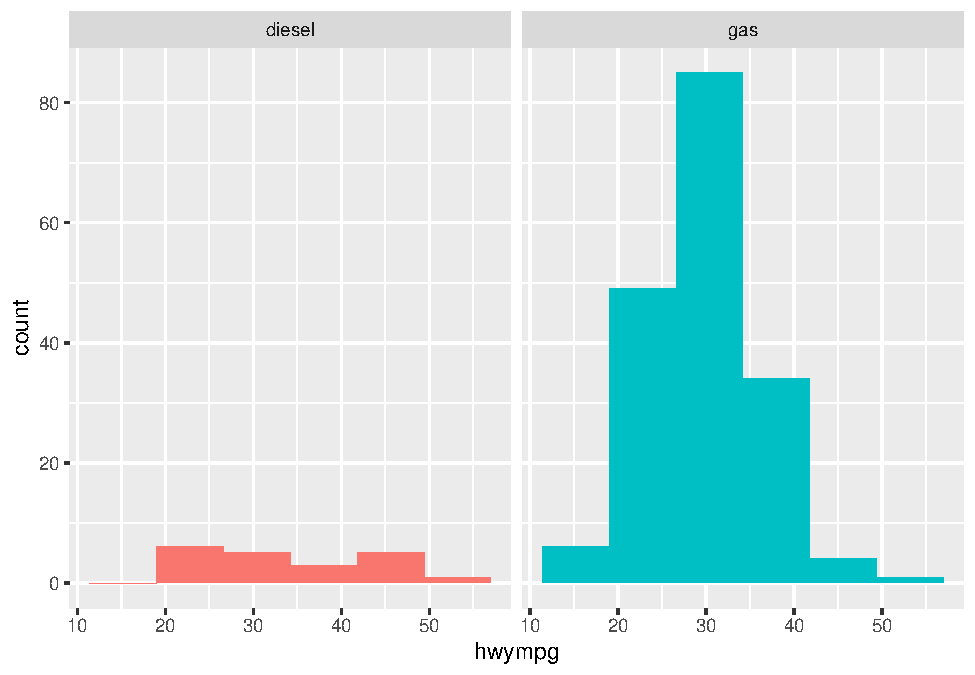
\includegraphics{project2_files/figure-latex/unnamed-chunk-2-1} \end{center}

\begin{Shaded}
\begin{Highlighting}[]
\NormalTok{autorand }\OperatorTok\StringTok{ }\KeywordTok{group_by}\NormalTok{(fueltype) }\OperatorTok\StringTok{ }\KeywordTok{summarize}\NormalTok{(}\DataTypeTok{means =} \KeywordTok{mean}\NormalTok{(hwympg)) }\OperatorTok\StringTok{ }
\StringTok{    }\KeywordTok{summarize}\NormalTok{(}\StringTok{`}\DataTypeTok{mean_diff:}\StringTok{`}\NormalTok{ =}\StringTok{ }\KeywordTok{diff}\NormalTok{(means)) }\OperatorTok\StringTok{ }\KeywordTok{glimpse}\NormalTok{()}
\end{Highlighting}
\end{Shaded}

\begin{verbatim}
## Observations: 1
## Variables: 1
## $ `mean_diff:` <dbl> -4.565642
\end{verbatim}

\begin{Shaded}
\begin{Highlighting}[]
\NormalTok{rand_wt <-}\StringTok{ }\KeywordTok{vector}\NormalTok{()}

\ControlFlowTok{for}\NormalTok{ (i }\ControlFlowTok{in} \DecValTok{1}\OperatorTok{:}\DecValTok{5000}\NormalTok{) \{}
\NormalTok{    new <-}\StringTok{ }\KeywordTok{data.frame}\NormalTok{(}\DataTypeTok{hwympg =} \KeywordTok{sample}\NormalTok{(autorand}\OperatorTok{$}\NormalTok{hwympg), }\DataTypeTok{condition =}\NormalTok{ autorand}\OperatorTok{$}\NormalTok{fueltype)}
\NormalTok{    rand_wt[i] <-}\StringTok{ }\KeywordTok{mean}\NormalTok{(new[new}\OperatorTok{$}\NormalTok{condition }\OperatorTok{==}\StringTok{ "gas"}\NormalTok{, ]}\OperatorTok{$}\NormalTok{hwympg) }\OperatorTok{-}\StringTok{ }
\StringTok{        }\KeywordTok{mean}\NormalTok{(new[new}\OperatorTok{$}\NormalTok{condition }\OperatorTok{==}\StringTok{ "diesel"}\NormalTok{, ]}\OperatorTok{$}\NormalTok{hwympg)}
\NormalTok{\}}

\CommentTok{# two-tailed p-value}
\KeywordTok{mean}\NormalTok{(rand_wt }\OperatorTok{>}\StringTok{ }\FloatTok{4.5656} \OperatorTok{|}\StringTok{ }\NormalTok{rand_wt }\OperatorTok{<}\StringTok{ }\FloatTok{-4.5656}\NormalTok{)}
\end{Highlighting}
\end{Shaded}

\begin{verbatim}
## [1] 0.0046
\end{verbatim}

\begin{Shaded}
\begin{Highlighting}[]
\CommentTok{# Plot}
\KeywordTok{library}\NormalTok{(vegan)}
\NormalTok{F_obs <-}\StringTok{ }\FloatTok{2.6878}

\NormalTok{Fs <-}\StringTok{ }\KeywordTok{replicate}\NormalTok{(}\DecValTok{5000}\NormalTok{, \{}
\NormalTok{    new <-}\StringTok{ }\NormalTok{Automobile }\OperatorTok\StringTok{ }\KeywordTok{mutate}\NormalTok{(}\DataTypeTok{highway.mpg =} \KeywordTok{sample}\NormalTok{(highway.mpg))}
\NormalTok{    SSW <-}\StringTok{ }\NormalTok{new }\OperatorTok\StringTok{ }\KeywordTok{group_by}\NormalTok{(fuel.type) }\OperatorTok\StringTok{ }\KeywordTok{summarize}\NormalTok{(}\DataTypeTok{SSW =} \KeywordTok{sum}\NormalTok{((highway.mpg }\OperatorTok{-}\StringTok{ }
\StringTok{        }\KeywordTok{mean}\NormalTok{(highway.mpg))}\OperatorTok{^}\DecValTok{2}\NormalTok{)) }\OperatorTok\StringTok{ }\KeywordTok{summarize}\NormalTok{(}\KeywordTok{sum}\NormalTok{(SSW)) }\OperatorTok\StringTok{ }\NormalTok{pull}
\NormalTok{    SSB <-}\StringTok{ }\NormalTok{new }\OperatorTok\StringTok{ }\KeywordTok{mutate}\NormalTok{(}\DataTypeTok{mean =} \KeywordTok{mean}\NormalTok{(highway.mpg)) }\OperatorTok\StringTok{ }\KeywordTok{group_by}\NormalTok{(fuel.type) }\OperatorTok\StringTok{ }
\StringTok{        }\KeywordTok{mutate}\NormalTok{(}\DataTypeTok{groupmean =} \KeywordTok{mean}\NormalTok{(highway.mpg)) }\OperatorTok\StringTok{ }\KeywordTok{summarize}\NormalTok{(}\DataTypeTok{SSB =} \KeywordTok{sum}\NormalTok{((mean }\OperatorTok{-}\StringTok{ }
\StringTok{        }\NormalTok{groupmean)}\OperatorTok{^}\DecValTok{2}\NormalTok{)) }\OperatorTok\StringTok{ }\KeywordTok{summarize}\NormalTok{(}\KeywordTok{sum}\NormalTok{(SSB)) }\OperatorTok\StringTok{ }\NormalTok{pull}
\NormalTok{    (SSB}\OperatorTok{/}\DecValTok{1}\NormalTok{)}\OperatorTok{/}\NormalTok{(SSW}\OperatorTok{/}\DecValTok{197}\NormalTok{)}
\NormalTok{\})}

\NormalTok{\{}
    \KeywordTok{hist}\NormalTok{(Fs, }\DataTypeTok{prob =}\NormalTok{ T)}
    \KeywordTok{abline}\NormalTok{(}\DataTypeTok{v =}\NormalTok{ F_obs, }\DataTypeTok{col =} \StringTok{"red"}\NormalTok{, }\DataTypeTok{add =}\NormalTok{ T)}
\NormalTok{\}}
\end{Highlighting}
\end{Shaded}

\begin{center}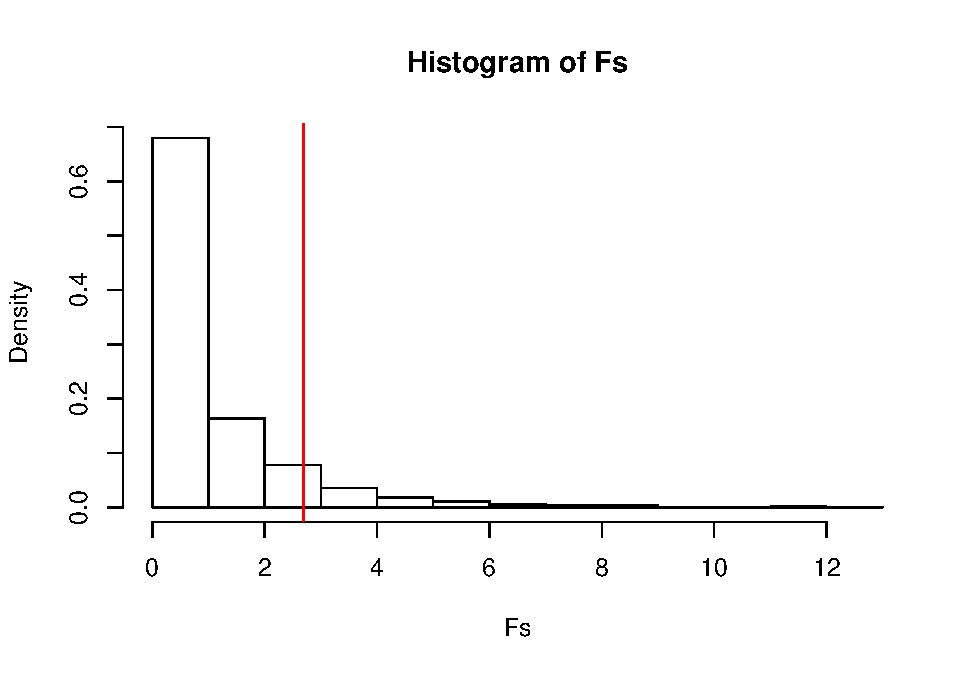
\includegraphics{project2_files/figure-latex/unnamed-chunk-2-2} \end{center}

I decided to test the association between fuel type and highway mpg, so
I conducted a randomization test and found the mean difference. My null
hypothesis was that the mean highway mpg is the same for gasoline and
diesel cars. Conversely, my alternative hypothesis was the mean highway
mpg is different for gasoline and diesel cars. Fuel type was a binary
categorical variable, so I found the mean difference in highway mpg
between gas and diesel cars. To begin, I created a dataframe of just
these two variables from the Automobile dataset, plotted it, and found
the actual mean difference between gas and diesel cars, which was
-4.5656 mpg. This suggests that on average, diesel cars get highway mpg
than gasoline cars by about 4.5656 mpg. I then completed 5000 random
permutations. After performing all of these computations and completing
the randomization test, I found the two-tailed p-value in order to
determine if the test statistic is large enough to suggest that the
association is not due to chance. The p-value determines the probability
of observing a mean difference as large as the one I computed for the
original data. The p-value was 0.0026. Because it was less than 0.05,
the null hypothesis was rejected. This means that highway mpg is
different for gasoline and diesel cars.

\subsection{3. Linear Regression Model}\label{linear-regression-model}

\begin{Shaded}
\begin{Highlighting}[]
\KeywordTok{library}\NormalTok{(tidyverse)}
\NormalTok{Automobile}\OperatorTok{$}\NormalTok{engine_c <-}\StringTok{ }\NormalTok{Automobile}\OperatorTok{$}\NormalTok{engine.size }\OperatorTok{-}\StringTok{ }\KeywordTok{mean}\NormalTok{(Automobile}\OperatorTok{$}\NormalTok{engine.size)}
\NormalTok{fit <-}\StringTok{ }\KeywordTok{lm}\NormalTok{(city.mpg }\OperatorTok{~}\StringTok{ }\NormalTok{body.style }\OperatorTok{*}\StringTok{ }\NormalTok{engine_c, }\DataTypeTok{data =}\NormalTok{ Automobile)}
\KeywordTok{summary}\NormalTok{(fit)}
\end{Highlighting}
\end{Shaded}

\begin{verbatim}
## 
## Call:
## lm(formula = city.mpg ~ body.style * engine_c, data = Automobile)
## 
## Residuals:
##      Min       1Q   Median       3Q      Max 
## -14.8172  -2.5325  -0.0596   1.9658  19.9658 
## 
## Coefficients:
##                              Estimate Std. Error t value Pr(>|t|)    
## (Intercept)                  22.46466    2.39811   9.368   <2e-16 ***
## body.stylehardtop             3.18795    3.28512   0.970    0.333    
## body.stylehatchback           2.24262    2.48105   0.904    0.367    
## body.stylesedan               3.07397    2.44901   1.255    0.211    
## body.stylewagon               1.33208    2.58258   0.516    0.607    
## engine_c                     -0.06346    0.04514  -1.406    0.161    
## body.stylehardtop:engine_c   -0.01702    0.05398  -0.315    0.753    
## body.stylehatchback:engine_c -0.06304    0.04946  -1.275    0.204    
## body.stylesedan:engine_c     -0.04132    0.04676  -0.884    0.378    
## body.stylewagon:engine_c     -0.03935    0.05790  -0.680    0.498    
## ---
## Signif. codes:  0 '***' 0.001 '**' 0.01 '*' 0.05 '.' 0.1 ' ' 1
## 
## Residual standard error: 4.773 on 189 degrees of freedom
## Multiple R-squared:  0.4353, Adjusted R-squared:  0.4085 
## F-statistic: 16.19 on 9 and 189 DF,  p-value: < 2.2e-16
\end{verbatim}

\begin{Shaded}
\begin{Highlighting}[]
\KeywordTok{summary}\NormalTok{(fit)}\OperatorTok{$}\NormalTok{coef}
\end{Highlighting}
\end{Shaded}

\begin{verbatim}
##                                 Estimate Std. Error    t value     Pr(>|t|)
## (Intercept)                  22.46466318 2.39811162  9.3676470 2.268429e-17
## body.stylehardtop             3.18795182 3.28511679  0.9704227 3.330761e-01
## body.stylehatchback           2.24261808 2.48104651  0.9039001 3.671991e-01
## body.stylesedan               3.07397352 2.44901122  1.2551896 2.109597e-01
## body.stylewagon               1.33208486 2.58257678  0.5157968 6.065992e-01
## engine_c                     -0.06345681 0.04514278 -1.4056911 1.614576e-01
## body.stylehardtop:engine_c   -0.01702472 0.05397682 -0.3154079 7.527999e-01
## body.stylehatchback:engine_c -0.06304016 0.04945679 -1.2746513 2.039976e-01
## body.stylesedan:engine_c     -0.04132187 0.04676126 -0.8836773 3.779931e-01
## body.stylewagon:engine_c     -0.03935336 0.05790117 -0.6796643 4.975486e-01
\end{verbatim}

\begin{Shaded}
\begin{Highlighting}[]
\CommentTok{# Linear Regression Plot}
\KeywordTok{library}\NormalTok{(ggplot2)}
\NormalTok{predict <-}\StringTok{ }\KeywordTok{predict}\NormalTok{(fit, Automobile)}
\KeywordTok{ggplot}\NormalTok{(Automobile, }\KeywordTok{aes}\NormalTok{(}\DataTypeTok{x =}\NormalTok{ engine_c, }\DataTypeTok{y =}\NormalTok{ city.mpg, }\DataTypeTok{group =}\NormalTok{ body.style)) }\OperatorTok{+}\StringTok{ }
\StringTok{    }\KeywordTok{geom_point}\NormalTok{(}\KeywordTok{aes}\NormalTok{(}\DataTypeTok{color =}\NormalTok{ body.style)) }\OperatorTok{+}\StringTok{ }\KeywordTok{geom_line}\NormalTok{(}\DataTypeTok{data =}\NormalTok{ Automobile, }
    \KeywordTok{aes}\NormalTok{(}\DataTypeTok{y =}\NormalTok{ predict, }\DataTypeTok{color =}\NormalTok{ body.style))}
\end{Highlighting}
\end{Shaded}

\begin{center}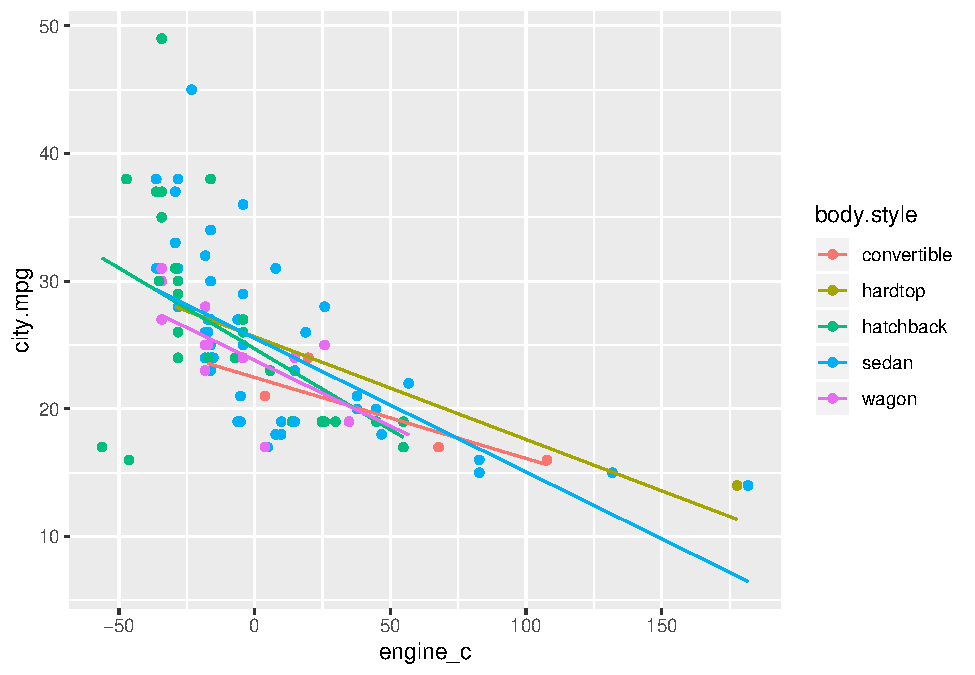
\includegraphics{project2_files/figure-latex/unnamed-chunk-3-1} \end{center}

\begin{Shaded}
\begin{Highlighting}[]
\KeywordTok{qplot}\NormalTok{(}\DataTypeTok{x =}\NormalTok{ engine_c, }\DataTypeTok{y =}\NormalTok{ city.mpg, }\DataTypeTok{color =}\NormalTok{ body.style, }\DataTypeTok{data =}\NormalTok{ Automobile) }\OperatorTok{+}\StringTok{ }
\StringTok{    }\KeywordTok{stat_smooth}\NormalTok{(}\DataTypeTok{method =} \StringTok{"lm"}\NormalTok{, }\DataTypeTok{se =} \OtherTok{FALSE}\NormalTok{, }\DataTypeTok{fullrange =} \OtherTok{TRUE}\NormalTok{)}
\end{Highlighting}
\end{Shaded}

\begin{center}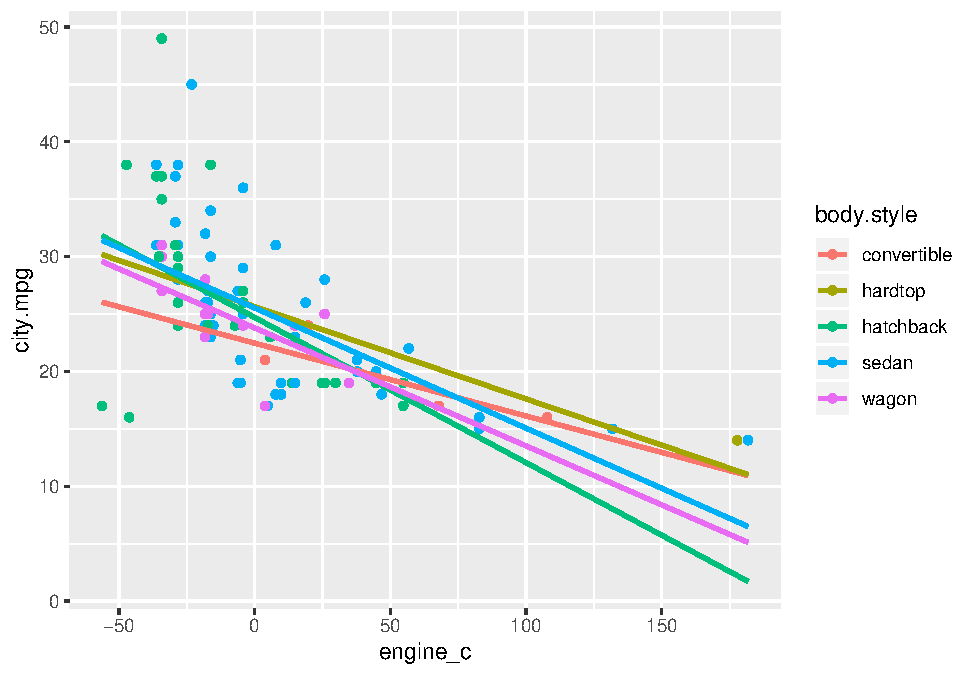
\includegraphics{project2_files/figure-latex/unnamed-chunk-3-2} \end{center}

\begin{Shaded}
\begin{Highlighting}[]
\CommentTok{# Checking linearity assumption with scatterplot}
\NormalTok{resids <-}\StringTok{ }\NormalTok{fit}\OperatorTok{$}\NormalTok{residuals}
\NormalTok{fitvals <-}\StringTok{ }\NormalTok{fit}\OperatorTok{$}\NormalTok{fitted.values}
\KeywordTok{ggplot}\NormalTok{() }\OperatorTok{+}\StringTok{ }\KeywordTok{geom_point}\NormalTok{(}\KeywordTok{aes}\NormalTok{(fitvals, resids)) }\OperatorTok{+}\StringTok{ }\KeywordTok{geom_hline}\NormalTok{(}\DataTypeTok{yintercept =} \DecValTok{0}\NormalTok{, }
    \DataTypeTok{color =} \StringTok{"red"}\NormalTok{)}
\end{Highlighting}
\end{Shaded}

\begin{center}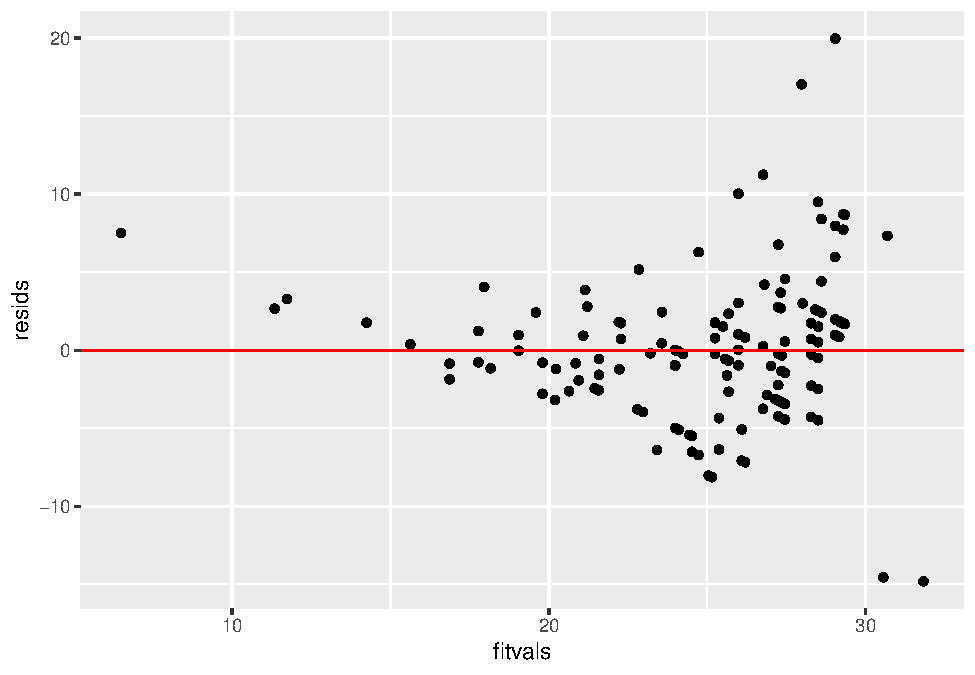
\includegraphics{project2_files/figure-latex/unnamed-chunk-3-3} \end{center}

\begin{Shaded}
\begin{Highlighting}[]
\CommentTok{# Checking assumption of homoskedasticity with Breuch-Pagan}
\CommentTok{# test}
\KeywordTok{library}\NormalTok{(dplyr)}
\KeywordTok{library}\NormalTok{(lmtest)}
\KeywordTok{library}\NormalTok{(sandwich)}
\KeywordTok{bptest}\NormalTok{(fit)}
\end{Highlighting}
\end{Shaded}

\begin{verbatim}
## 
##  studentized Breusch-Pagan test
## 
## data:  fit
## BP = 27.322, df = 9, p-value = 0.001237
\end{verbatim}

\begin{Shaded}
\begin{Highlighting}[]
\CommentTok{# Checking normality assumption with Shapiro-Wilk test and}
\CommentTok{# graphs}
\KeywordTok{shapiro.test}\NormalTok{(resids)}
\end{Highlighting}
\end{Shaded}

\begin{verbatim}
## 
##  Shapiro-Wilk normality test
## 
## data:  resids
## W = 0.946, p-value = 8.373e-07
\end{verbatim}

\begin{Shaded}
\begin{Highlighting}[]
\KeywordTok{ggplot}\NormalTok{() }\OperatorTok{+}\StringTok{ }\KeywordTok{geom_histogram}\NormalTok{(}\KeywordTok{aes}\NormalTok{(resids), }\DataTypeTok{bins =} \DecValTok{20}\NormalTok{)}
\end{Highlighting}
\end{Shaded}

\begin{center}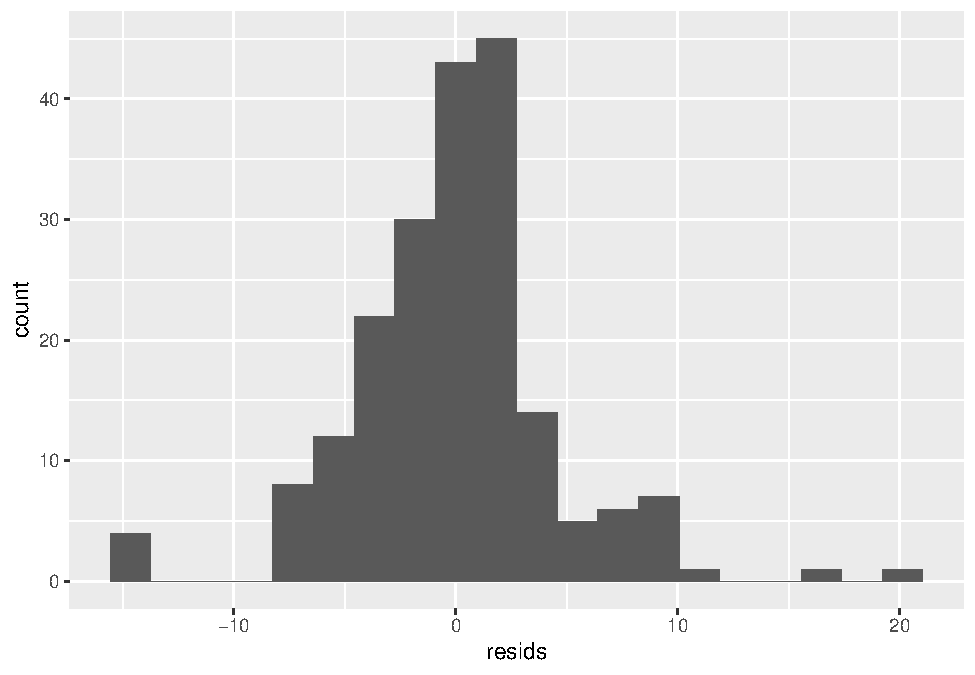
\includegraphics{project2_files/figure-latex/unnamed-chunk-3-4} \end{center}

\begin{Shaded}
\begin{Highlighting}[]
\CommentTok{# Robust Standard Errors}
\KeywordTok{coeftest}\NormalTok{(fit, }\DataTypeTok{vcov =} \KeywordTok{vcovHC}\NormalTok{(fit))}
\end{Highlighting}
\end{Shaded}

\begin{verbatim}
## 
## t test of coefficients:
## 
##                               Estimate Std. Error t value  Pr(>|t|)    
## (Intercept)                  22.464663   0.898512 25.0021 < 2.2e-16 ***
## body.stylehardtop             3.187952   2.107921  1.5124  0.132111    
## body.stylehatchback           2.242618   1.009919  2.2206  0.027567 *  
## body.stylesedan               3.073974   1.025964  2.9962  0.003101 ** 
## body.stylewagon               1.332085   1.131754  1.1770  0.240672    
## engine_c                     -0.063457   0.012298 -5.1598 6.221e-07 ***
## body.stylehardtop:engine_c   -0.017025   0.056045 -0.3038  0.761639    
## body.stylehatchback:engine_c -0.063040   0.029370 -2.1464  0.033114 *  
## body.stylesedan:engine_c     -0.041322   0.018523 -2.2309  0.026866 *  
## body.stylewagon:engine_c     -0.039353   0.028933 -1.3602  0.175398    
## ---
## Signif. codes:  0 '***' 0.001 '**' 0.01 '*' 0.05 '.' 0.1 ' ' 1
\end{verbatim}

I performed a multiple regression test to see the effects of body style,
engine size, and the interaction between the two on city mpg. In
context, the intercept shows that the predicted city mpg for a
convertible with an average engine size is 22.464 mpg. In cars with
average engine size, city mpg is 3.188 mpg higher for hardtops than for
convertibles, 2.24 mpg higher for hatchbacks, 3.07 mpg higher for
sedans, and 1.33 mpg higher for wagons than for convertibles.
Convertibles show a decrease of 0.06 mpg in city mpg for every 1-unit
increase in engine size on average. The slope for engine size on city
mpg is 0.017 less for hardtops compared to convertibles, 0.063 less for
hatchbacks compared to convertibles, 0.041 less for sedans compared to
convertibles, and 0.039 less for wagons compared to convertibles. The R
squared is 0.4353, which means that 43.53\% of variation in the outcome
is explained by this model. The adjusted R squared is basically a
penalty for capitalizing on chance and is therefore slightly lower at
0.4085. After interpreting the coefficient estimates, I plotted the
regression using ggplot and then checked the assumptions of linearity,
normality, and homoskedasticity. I checked linearity and
homoskedasticity by graphing residuals on a scatterplot, and the data
points appeared to fan out in the plot and appeared to depart from
fitted noise, so this seems to violate both assumptions. I then formally
tested homoskedasticity with a Breuch-Pagan test. The null hypothesis of
the BP test was that the distribution was homoskedastic, but because the
p-value was smaller than 0.05, this hypothesis was rejected. Finally, I
created a histogram and found that the distribution looked pretty mound
shaped and therefore normal. I formally tested normality with the
Shapiro-Wilk test, and because the p-value was much smaller than 0.05,
the null hypothesis stating that the true distribution is normal was
rejected. The assumptions of linearity, homoskedasticity, and normality
were not met. Because the distribution was heteroskedastic, robust
standard errors were used. With these new regression results, 6 of the
coefficient estimates were significant: the intercept, hatchback body
style, sedan body style, engine\_c, the interaction between hatchback
body style and engine\_c, and the interaction between sedan and
engine\_c. This is different from the test when robust SEs were not used
because only the intercept was significant before, whereas with robust
SEs, five additional estimates are significant.

\subsection{4. Bootstrapped Standard
Errors}\label{bootstrapped-standard-errors}

\begin{Shaded}
\begin{Highlighting}[]
\NormalTok{sample <-}\StringTok{ }\KeywordTok{replicate}\NormalTok{(}\DecValTok{5000}\NormalTok{, \{}
\NormalTok{    boot <-}\StringTok{ }\NormalTok{Automobile[}\KeywordTok{sample}\NormalTok{(}\KeywordTok{nrow}\NormalTok{(Automobile), }\DataTypeTok{replace =} \OtherTok{TRUE}\NormalTok{), }
\NormalTok{        ]}
\NormalTok{    fit2 <-}\StringTok{ }\KeywordTok{lm}\NormalTok{(city.mpg }\OperatorTok{~}\StringTok{ }\NormalTok{body.style }\OperatorTok{*}\StringTok{ }\NormalTok{engine_c, }\DataTypeTok{data =}\NormalTok{ boot)}
    \KeywordTok{coef}\NormalTok{(fit2)}
    
\NormalTok{\})}
\KeywordTok{do.call}\NormalTok{(rbind, sample) }\OperatorTok\StringTok{ }\NormalTok{as.data.frame }\OperatorTok\StringTok{ }\KeywordTok{summarize_all}\NormalTok{(sd, }
    \DataTypeTok{na.rm =}\NormalTok{ T)}
\end{Highlighting}
\end{Shaded}

\begin{verbatim}
##   (Intercept) body.stylehardtop body.stylehatchback body.stylesedan
## 1    1.128948          2.203575            1.214948         1.24381
##   body.stylewagon  engine_c body.stylehardtop:engine_c
## 1        1.328604 0.0480374                 0.06024269
##   body.stylehatchback:engine_c body.stylesedan:engine_c
## 1                   0.05516711                0.8488794
##   body.stylewagon:engine_c
## 1                0.1036326
\end{verbatim}

I reran the same regression model with interaction as before, but this
time I computed bootstrapped standard errors. Bootstrapped standard
errors were used because my distribution was not normal. The bootstrap
SEs decreased from the normal standard errors in the intercept and all
of the body styles. The bootstrap SEs increased in the engine\_c and all
of the interaction categories. The bootstrap SEs increased in every
category from the robust standard errors. All of the other bootstrap SEs
decreased from the robust standard errors. Overall, it appears that the
bootstrap errors worked as well as the normal standard errors but worse
than the robust standard errors.

\subsection{5. Logistic Regression}\label{logistic-regression}

\begin{Shaded}
\begin{Highlighting}[]
\KeywordTok{library}\NormalTok{(tidyverse)}
\KeywordTok{library}\NormalTok{(lmtest)}
\NormalTok{data <-}\StringTok{ }\NormalTok{Automobile }\OperatorTok\StringTok{ }\KeywordTok{mutate}\NormalTok{(}\DataTypeTok{y =} \KeywordTok{ifelse}\NormalTok{(fuel.type }\OperatorTok{==}\StringTok{ "gas"}\NormalTok{, }
    \DecValTok{1}\NormalTok{, }\DecValTok{0}\NormalTok{))}
\KeywordTok{head}\NormalTok{(data)}
\end{Highlighting}
\end{Shaded}

\begin{verbatim}
## # A tibble: 6 x 8
##   fuel.type body.style num.of.cylinders engine.size city.mpg highway.mpg
##   <chr>     <chr>      <chr>                  <dbl>    <dbl>       <dbl>
## 1 gas       convertib~ four                     130       21          27
## 2 gas       convertib~ four                     130       21          27
## 3 gas       hatchback  six                      152       19          26
## 4 gas       sedan      four                     109       24          30
## 5 gas       sedan      five                     136       18          22
## 6 gas       sedan      five                     136       19          25
## # ... with 2 more variables: engine_c <dbl>, y <dbl>
\end{verbatim}

\begin{Shaded}
\begin{Highlighting}[]
\NormalTok{fit3 <-}\StringTok{ }\KeywordTok{glm}\NormalTok{(y }\OperatorTok{~}\StringTok{ }\NormalTok{engine.size }\OperatorTok{+}\StringTok{ }\NormalTok{city.mpg, }\DataTypeTok{data =}\NormalTok{ data, }\DataTypeTok{family =} \KeywordTok{binomial}\NormalTok{(}\DataTypeTok{link =} \StringTok{"logit"}\NormalTok{))}
\KeywordTok{coeftest}\NormalTok{(fit3)}
\end{Highlighting}
\end{Shaded}

\begin{verbatim}
## 
## z test of coefficients:
## 
##               Estimate Std. Error z value  Pr(>|z|)    
## (Intercept) 17.4260343  3.1769391  5.4852 4.131e-08 ***
## engine.size -0.0443786  0.0097614 -4.5463 5.459e-06 ***
## city.mpg    -0.3495505  0.0709001 -4.9302 8.215e-07 ***
## ---
## Signif. codes:  0 '***' 0.001 '**' 0.01 '*' 0.05 '.' 0.1 ' ' 1
\end{verbatim}

\begin{Shaded}
\begin{Highlighting}[]
\KeywordTok{exp}\NormalTok{(}\KeywordTok{coef}\NormalTok{(fit3))}
\end{Highlighting}
\end{Shaded}

\begin{verbatim}
##  (Intercept)  engine.size     city.mpg 
## 3.698542e+07 9.565917e-01 7.050049e-01
\end{verbatim}

\begin{Shaded}
\begin{Highlighting}[]
\CommentTok{# Confusion Matrix}
\NormalTok{Automobile}\OperatorTok{$}\NormalTok{predict <-}\StringTok{ }\KeywordTok{predict}\NormalTok{(fit3, }\DataTypeTok{data =}\NormalTok{ Automobile, }\DataTypeTok{type =} \StringTok{"response"}\NormalTok{)}
\KeywordTok{table}\NormalTok{(}\DataTypeTok{predict =} \KeywordTok{as.numeric}\NormalTok{(Automobile}\OperatorTok{$}\NormalTok{predict }\OperatorTok{>}\StringTok{ }\FloatTok{0.5}\NormalTok{), }\DataTypeTok{truth =}\NormalTok{ Automobile}\OperatorTok{$}\NormalTok{fuel.type) }\OperatorTok\StringTok{ }
\StringTok{    }\NormalTok{addmargins}
\end{Highlighting}
\end{Shaded}

\begin{verbatim}
##        truth
## predict diesel gas Sum
##     0        3   4   7
##     1       17 175 192
##     Sum     20 179 199
\end{verbatim}

\begin{Shaded}
\begin{Highlighting}[]
\CommentTok{# Accuracy}
\NormalTok{(}\DecValTok{3} \OperatorTok{+}\StringTok{ }\DecValTok{175}\NormalTok{)}\OperatorTok{/}\DecValTok{199}
\end{Highlighting}
\end{Shaded}

\begin{verbatim}
## [1] 0.8944724
\end{verbatim}

\begin{Shaded}
\begin{Highlighting}[]
\CommentTok{# Sensitivity (TPR)}
\DecValTok{175}\OperatorTok{/}\DecValTok{179}
\end{Highlighting}
\end{Shaded}

\begin{verbatim}
## [1] 0.9776536
\end{verbatim}

\begin{Shaded}
\begin{Highlighting}[]
\CommentTok{# Specificity (TNR)}
\DecValTok{3}\OperatorTok{/}\DecValTok{20}
\end{Highlighting}
\end{Shaded}

\begin{verbatim}
## [1] 0.15
\end{verbatim}

\begin{Shaded}
\begin{Highlighting}[]
\CommentTok{# Recall (PPV)}
\DecValTok{175}\OperatorTok{/}\DecValTok{192}
\end{Highlighting}
\end{Shaded}

\begin{verbatim}
## [1] 0.9114583
\end{verbatim}

\begin{Shaded}
\begin{Highlighting}[]
\CommentTok{# Density Plot}
\NormalTok{logit <-}\StringTok{ }\KeywordTok{predict}\NormalTok{(fit3)}
\NormalTok{Automobile }\OperatorTok\StringTok{ }\KeywordTok{ggplot}\NormalTok{() }\OperatorTok{+}\StringTok{ }\KeywordTok{geom_density}\NormalTok{(}\KeywordTok{aes}\NormalTok{(logit, }\DataTypeTok{color =}\NormalTok{ fuel.type, }
    \DataTypeTok{fill =}\NormalTok{ fuel.type), }\DataTypeTok{alpha =} \FloatTok{0.4}\NormalTok{) }\OperatorTok{+}\StringTok{ }\KeywordTok{theme}\NormalTok{(}\DataTypeTok{legend.position =} \KeywordTok{c}\NormalTok{(}\FloatTok{0.85}\NormalTok{, }
    \FloatTok{0.85}\NormalTok{)) }\OperatorTok{+}\StringTok{ }\KeywordTok{geom_vline}\NormalTok{(}\DataTypeTok{xintercept =} \DecValTok{0}\NormalTok{) }\OperatorTok{+}\StringTok{ }\KeywordTok{xlab}\NormalTok{(}\StringTok{"predictor (logit)"}\NormalTok{)}
\end{Highlighting}
\end{Shaded}

\begin{center}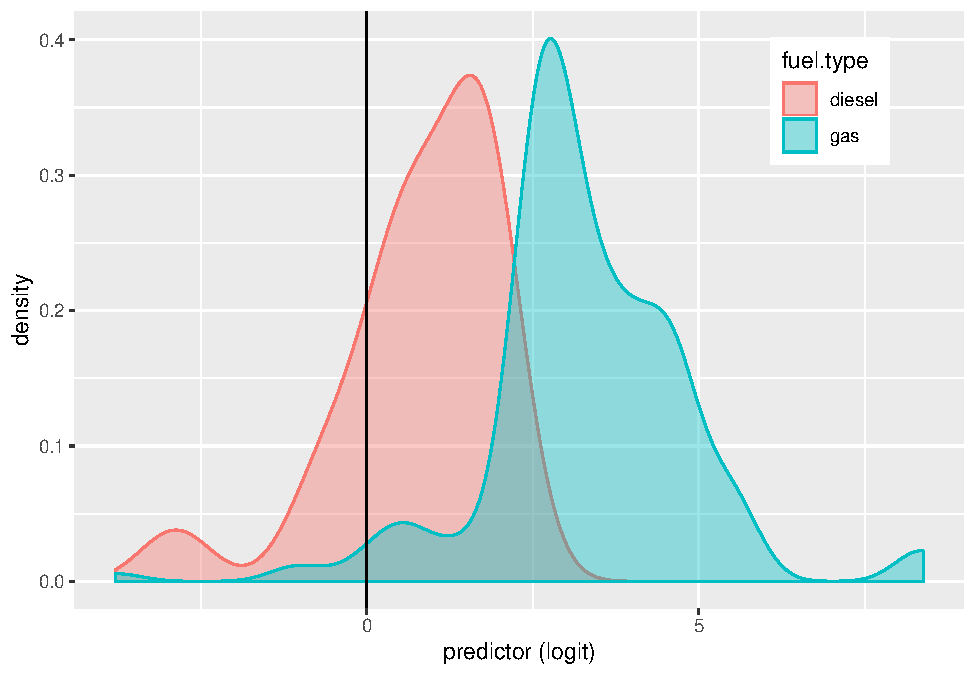
\includegraphics{project2_files/figure-latex/unnamed-chunk-5-1} \end{center}

\begin{Shaded}
\begin{Highlighting}[]
\CommentTok{# ROC Plot and AUC}
\KeywordTok{library}\NormalTok{(pROC)}
\KeywordTok{library}\NormalTok{(plotROC)}
\NormalTok{ROC0 <-}\StringTok{ }\NormalTok{Automobile }\OperatorTok\StringTok{ }\KeywordTok{mutate}\NormalTok{(}\DataTypeTok{prob =} \KeywordTok{predict}\NormalTok{(fit3, }\DataTypeTok{type =} \StringTok{"response"}\NormalTok{), }
    \DataTypeTok{prediction =} \KeywordTok{ifelse}\NormalTok{(prob }\OperatorTok{>}\StringTok{ }\FloatTok{0.5}\NormalTok{, }\DecValTok{1}\NormalTok{, }\DecValTok{0}\NormalTok{))}
\NormalTok{ROC1 <-}\StringTok{ }\NormalTok{ROC0 }\OperatorTok\StringTok{ }\KeywordTok{transmute}\NormalTok{(prob, predict, }\DataTypeTok{truth =}\NormalTok{ fuel.type)}
\NormalTok{ROCplot <-}\StringTok{ }\KeywordTok{ggplot}\NormalTok{(ROC1) }\OperatorTok{+}\StringTok{ }\KeywordTok{geom_roc}\NormalTok{(}\KeywordTok{aes}\NormalTok{(}\DataTypeTok{d =}\NormalTok{ truth, }\DataTypeTok{m =}\NormalTok{ prob), }
    \DataTypeTok{n.cuts =} \DecValTok{0}\NormalTok{) }\OperatorTok{+}\StringTok{ }\KeywordTok{geom_segment}\NormalTok{(}\KeywordTok{aes}\NormalTok{(}\DataTypeTok{x =} \DecValTok{0}\NormalTok{, }\DataTypeTok{xend =} \DecValTok{1}\NormalTok{, }\DataTypeTok{y =} \DecValTok{0}\NormalTok{, }\DataTypeTok{yend =} \DecValTok{1}\NormalTok{), }
    \DataTypeTok{lty =} \DecValTok{2}\NormalTok{)}
\NormalTok{ROCplot}
\end{Highlighting}
\end{Shaded}

\begin{center}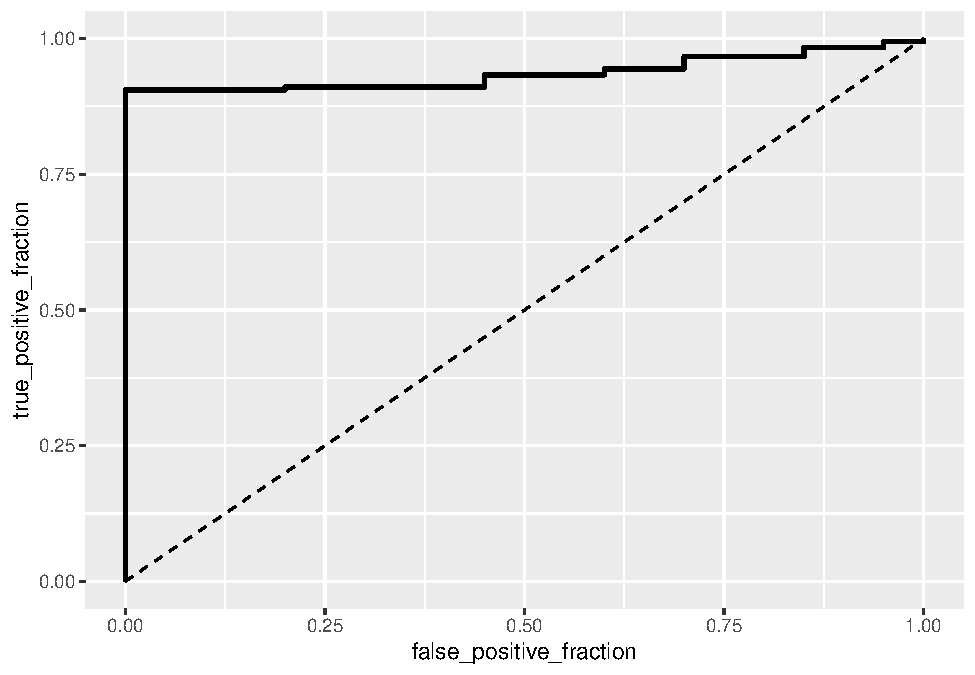
\includegraphics{project2_files/figure-latex/unnamed-chunk-5-2} \end{center}

\begin{Shaded}
\begin{Highlighting}[]
\KeywordTok{calc_auc}\NormalTok{(ROCplot)}
\end{Highlighting}
\end{Shaded}

\begin{verbatim}
##   PANEL group       AUC
## 1     1    -1 0.9360335
\end{verbatim}

\begin{Shaded}
\begin{Highlighting}[]
\CommentTok{# 10-Fold CV}
\KeywordTok{library}\NormalTok{(tidyverse)}
\KeywordTok{library}\NormalTok{(lmtest)}
\NormalTok{auto <-}\StringTok{ }\NormalTok{Automobile }\OperatorTok\StringTok{ }\KeywordTok{mutate}\NormalTok{(}\DataTypeTok{y =} \KeywordTok{ifelse}\NormalTok{(fuel.type }\OperatorTok{==}\StringTok{ "gas"}\NormalTok{, }
    \DecValTok{1}\NormalTok{, }\DecValTok{0}\NormalTok{))}
\NormalTok{auto}\OperatorTok{$}\NormalTok{outcome <-}\StringTok{ }\OtherTok{NULL}
\NormalTok{fit4 <-}\StringTok{ }\KeywordTok{glm}\NormalTok{(y }\OperatorTok{~}\StringTok{ }\NormalTok{., }\DataTypeTok{data =}\NormalTok{ auto, }\DataTypeTok{family =} \StringTok{"binomial"}\NormalTok{)}
\NormalTok{probs <-}\StringTok{ }\KeywordTok{predict}\NormalTok{(fit4, }\DataTypeTok{type =} \StringTok{"response"}\NormalTok{)}

\NormalTok{class_diag <-}\StringTok{ }\ControlFlowTok{function}\NormalTok{(probs, truth) \{}
    \ControlFlowTok{if}\NormalTok{ (}\KeywordTok{is.numeric}\NormalTok{(truth) }\OperatorTok{==}\StringTok{ }\OtherTok{FALSE} \OperatorTok{&}\StringTok{ }\KeywordTok{is.logical}\NormalTok{(truth) }\OperatorTok{==}\StringTok{ }\OtherTok{FALSE}\NormalTok{) }
\NormalTok{        truth <-}\StringTok{ }\KeywordTok{as.numeric}\NormalTok{(truth) }\OperatorTok{-}\StringTok{ }\DecValTok{1}
\NormalTok{    tab <-}\StringTok{ }\KeywordTok{table}\NormalTok{(}\KeywordTok{factor}\NormalTok{(probs }\OperatorTok{>}\StringTok{ }\FloatTok{0.5}\NormalTok{, }\DataTypeTok{levels =} \KeywordTok{c}\NormalTok{(}\StringTok{"FALSE"}\NormalTok{, }\StringTok{"TRUE"}\NormalTok{)), }
\NormalTok{        truth)}
\NormalTok{    prediction <-}\StringTok{ }\KeywordTok{ifelse}\NormalTok{(probs }\OperatorTok{>}\StringTok{ }\FloatTok{0.5}\NormalTok{, }\DecValTok{1}\NormalTok{, }\DecValTok{0}\NormalTok{)}
\NormalTok{    acc =}\StringTok{ }\KeywordTok{mean}\NormalTok{(truth }\OperatorTok{==}\StringTok{ }\NormalTok{prediction)}
\NormalTok{    sens =}\StringTok{ }\KeywordTok{mean}\NormalTok{(prediction[truth }\OperatorTok{==}\StringTok{ }\DecValTok{1}\NormalTok{] }\OperatorTok{==}\StringTok{ }\DecValTok{1}\NormalTok{)}
\NormalTok{    spec =}\StringTok{ }\KeywordTok{mean}\NormalTok{(prediction[truth }\OperatorTok{==}\StringTok{ }\DecValTok{0}\NormalTok{] }\OperatorTok{==}\StringTok{ }\DecValTok{0}\NormalTok{)}
\NormalTok{    ppv =}\StringTok{ }\KeywordTok{mean}\NormalTok{(truth[prediction }\OperatorTok{==}\StringTok{ }\DecValTok{1}\NormalTok{] }\OperatorTok{==}\StringTok{ }\DecValTok{1}\NormalTok{)}
    \CommentTok{# CALCULATE EXACT AUC}
\NormalTok{    ord <-}\StringTok{ }\KeywordTok{order}\NormalTok{(probs, }\DataTypeTok{decreasing =} \OtherTok{TRUE}\NormalTok{)}
\NormalTok{    probs <-}\StringTok{ }\NormalTok{probs[ord]}
\NormalTok{    truth <-}\StringTok{ }\NormalTok{truth[ord]}
\NormalTok{    TPR =}\StringTok{ }\KeywordTok{cumsum}\NormalTok{(truth)}\OperatorTok{/}\KeywordTok{max}\NormalTok{(}\DecValTok{1}\NormalTok{, }\KeywordTok{sum}\NormalTok{(truth))}
\NormalTok{    FPR =}\StringTok{ }\KeywordTok{cumsum}\NormalTok{(}\OperatorTok{!}\NormalTok{truth)}\OperatorTok{/}\KeywordTok{max}\NormalTok{(}\DecValTok{1}\NormalTok{, }\KeywordTok{sum}\NormalTok{(}\OperatorTok{!}\NormalTok{truth))}
\NormalTok{    dup <-}\StringTok{ }\KeywordTok{c}\NormalTok{(probs[}\OperatorTok{-}\DecValTok{1}\NormalTok{] }\OperatorTok{>=}\StringTok{ }\NormalTok{probs[}\OperatorTok{-}\KeywordTok{length}\NormalTok{(probs)], }\OtherTok{FALSE}\NormalTok{)}
\NormalTok{    TPR <-}\StringTok{ }\KeywordTok{c}\NormalTok{(}\DecValTok{0}\NormalTok{, TPR[}\OperatorTok{!}\NormalTok{dup], }\DecValTok{1}\NormalTok{)}
\NormalTok{    FPR <-}\StringTok{ }\KeywordTok{c}\NormalTok{(}\DecValTok{0}\NormalTok{, FPR[}\OperatorTok{!}\NormalTok{dup], }\DecValTok{1}\NormalTok{)}
\NormalTok{    n <-}\StringTok{ }\KeywordTok{length}\NormalTok{(TPR)}
\NormalTok{    auc <-}\StringTok{ }\KeywordTok{sum}\NormalTok{(((TPR[}\OperatorTok{-}\DecValTok{1}\NormalTok{] }\OperatorTok{+}\StringTok{ }\NormalTok{TPR[}\OperatorTok{-}\NormalTok{n])}\OperatorTok{/}\DecValTok{2}\NormalTok{) }\OperatorTok{*}\StringTok{ }\NormalTok{(FPR[}\OperatorTok{-}\DecValTok{1}\NormalTok{] }\OperatorTok{-}\StringTok{ }\NormalTok{FPR[}\OperatorTok{-}\NormalTok{n]))}
    \KeywordTok{data.frame}\NormalTok{(acc, sens, spec, ppv, auc)}
\NormalTok{\}}

\CommentTok{# 10-fold}
\KeywordTok{set.seed}\NormalTok{(}\DecValTok{1234}\NormalTok{)}
\NormalTok{k =}\StringTok{ }\DecValTok{10}
\NormalTok{data <-}\StringTok{ }\NormalTok{auto[}\KeywordTok{sample}\NormalTok{(}\KeywordTok{nrow}\NormalTok{(auto)), ]}
\NormalTok{folds <-}\StringTok{ }\KeywordTok{cut}\NormalTok{(}\KeywordTok{seq}\NormalTok{(}\DecValTok{1}\OperatorTok{:}\KeywordTok{nrow}\NormalTok{(auto)), }\DataTypeTok{breaks =}\NormalTok{ k, }\DataTypeTok{labels =}\NormalTok{ F)}
\NormalTok{diags <-}\StringTok{ }\OtherTok{NULL}
\ControlFlowTok{for}\NormalTok{ (i }\ControlFlowTok{in} \DecValTok{1}\OperatorTok{:}\NormalTok{k) \{}
\NormalTok{    train <-}\StringTok{ }\NormalTok{data[folds }\OperatorTok{!=}\StringTok{ }\NormalTok{i, ]}
\NormalTok{    test <-}\StringTok{ }\NormalTok{data[folds }\OperatorTok{==}\StringTok{ }\NormalTok{i, ]}
\NormalTok{    truth <-}\StringTok{ }\NormalTok{test}\OperatorTok{$}\NormalTok{y}
\NormalTok{    fit5 <-}\StringTok{ }\KeywordTok{glm}\NormalTok{(y }\OperatorTok{~}\StringTok{ }\NormalTok{engine.size }\OperatorTok{+}\StringTok{ }\NormalTok{city.mpg, }\DataTypeTok{data =}\NormalTok{ train, }\DataTypeTok{family =} \StringTok{"binomial"}\NormalTok{)}
\NormalTok{    probs1 <-}\StringTok{ }\KeywordTok{predict}\NormalTok{(fit5, }\DataTypeTok{newdata =}\NormalTok{ test, }\DataTypeTok{type =} \StringTok{"response"}\NormalTok{)}
\NormalTok{    diags <-}\StringTok{ }\KeywordTok{rbind}\NormalTok{(diags, }\KeywordTok{class_diag}\NormalTok{(probs1, truth))}
\NormalTok{\}}
\KeywordTok{summarize_all}\NormalTok{(diags, mean)}
\end{Highlighting}
\end{Shaded}

\begin{verbatim}
##         acc      sens spec       ppv       auc
## 1 0.8847368 0.9667105  NaN 0.9114035 0.9342492
\end{verbatim}

Controlling for city mpg, there is a significant effect of engine size
on fuel type. Likewise, controlling for engine size, there is a
significant effect of city mpg on fuel type. In other words, a car's
fuel type can be predicted from its engine size and city mpg. Because
these estimates are both negative, as engine size and city mpg increase,
the odds that the car's fuel type is gasoline decreases. When engine
size and city-mpg are equal to 0, the odds that the car's fuel type is
gasoline is high. This means that the smaller the engine size and the
less city mpg, the more likely the car uses gasoline. Every one unit
increase in engine size decreases the odds of a gasoline fuel type by a
factor of 0.957 and every one unit increase in city mpg decreases the
odds by a factor of 0.705. I then created a confusion matrix. In the
confusion matrix, I see 4 false negatives and 17 false positives. Out of
the 179 gasoline cars, the model predicted 175, so the TPR, which
determines the proportion of gasoline cars correctly classified, is
0.9777. Out of the 20 cars that were not gasoline,the model predicted 3,
so the TNR is 0.15. The TNR is the proportion of diesel cars correctly
classified. Out of the 192 cars classified as gasoline by the model,
only 175 were, so the PPV, which determines the proportion of classified
gasoline cars that actually are gasoline, is 0.9115. The total accuracy,
which is proportion of correctly classified cases, is 0.8945. The TPR,
PPV, and accuracy are all pretty good, but the TNR is very low. The
density plot gives a visual representation of the classifications--the
gray has been misclassified. Right of 0, the gray area proportion
represents the false positives, or diesel cars that we predicted
gasoline. Left of 0, the gray area proportion represents the false
negatives, or gasoline cars that we predicted diesel. The red area
represents the correctly classified diesel cars and the blue area
represents the correctly classified gasoline cars. I calculated the ROC
plot next and AUC, which both looked pretty good. The AUC is 0.936,
which is the the area under the curve. This demonstrates that the model
is performing very well per AUC. After performing the 10-fold CV, I
obtained an out-of-sample accuracy of 0.885, sensitivity of 0.967, and
recall of 0.934. The recall from the 10-fold CV improved from above, but
decreased in accuracy and sensitivity.

\subsection{6. LASSO regression}\label{lasso-regression}

\begin{Shaded}
\begin{Highlighting}[]
\KeywordTok{library}\NormalTok{(glmnet)}
\NormalTok{y <-}\StringTok{ }\KeywordTok{as.matrix}\NormalTok{(Automobile}\OperatorTok{$}\NormalTok{fuel.type)}
\NormalTok{x <-}\StringTok{ }\KeywordTok{model.matrix}\NormalTok{(fuel.type }\OperatorTok{~}\StringTok{ }\NormalTok{., }\DataTypeTok{data =}\NormalTok{ Automobile)[, }\DecValTok{-1}\NormalTok{]}
\KeywordTok{head}\NormalTok{(x)}
\end{Highlighting}
\end{Shaded}

\begin{verbatim}
##   body.stylehardtop body.stylehatchback body.stylesedan body.stylewagon
## 1                 0                   0               0               0
## 2                 0                   0               0               0
## 3                 0                   1               0               0
## 4                 0                   0               1               0
## 5                 0                   0               1               0
## 6                 0                   0               1               0
##   num.of.cylindersfive num.of.cylindersfour num.of.cylinderssix
## 1                    0                    1                   0
## 2                    0                    1                   0
## 3                    0                    0                   1
## 4                    0                    1                   0
## 5                    1                    0                   0
## 6                    1                    0                   0
##   num.of.cylinderstwo engine.size city.mpg highway.mpg  engine_c   predict
## 1                   0         130       21          27   3.79397 0.9868261
## 2                   0         130       21          27   3.79397 0.9868261
## 3                   0         152       19          26  25.79397 0.9826903
## 4                   0         109       24          30 -17.20603 0.9852195
## 5                   0         136       18          22   9.79397 0.9939320
## 6                   0         136       19          25   9.79397 0.9914147
\end{verbatim}

\begin{Shaded}
\begin{Highlighting}[]
\NormalTok{x <-}\StringTok{ }\KeywordTok{scale}\NormalTok{(x)}
\NormalTok{cv <-}\StringTok{ }\KeywordTok{cv.glmnet}\NormalTok{(x, y, }\DataTypeTok{family =} \StringTok{"binomial"}\NormalTok{)}
\NormalTok{lasso <-}\StringTok{ }\KeywordTok{glmnet}\NormalTok{(x, y, }\DataTypeTok{family =} \StringTok{"binomial"}\NormalTok{, }\DataTypeTok{lambda =}\NormalTok{ cv}\OperatorTok{$}\NormalTok{lambda}\FloatTok{.1}\NormalTok{se)}
\KeywordTok{coef}\NormalTok{(lasso)}
\end{Highlighting}
\end{Shaded}

\begin{verbatim}
## 14 x 1 sparse Matrix of class "dgCMatrix"
##                              s0
## (Intercept)           2.6536710
## body.stylehardtop     .        
## body.stylehatchback   0.5403613
## body.stylesedan       .        
## body.stylewagon       .        
## num.of.cylindersfive -0.3902034
## num.of.cylindersfour  .        
## num.of.cylinderssix   .        
## num.of.cylinderstwo   .        
## engine.size           .        
## city.mpg             -0.2925875
## highway.mpg           .        
## engine_c              .        
## predict               0.6942446
\end{verbatim}

\begin{Shaded}
\begin{Highlighting}[]
\CommentTok{# 10-Fold CV}

\KeywordTok{set.seed}\NormalTok{(}\DecValTok{1234}\NormalTok{)}
\NormalTok{k =}\StringTok{ }\DecValTok{10}
\NormalTok{data <-}\StringTok{ }\NormalTok{auto[}\KeywordTok{sample}\NormalTok{(}\KeywordTok{nrow}\NormalTok{(auto)), ]}
\NormalTok{folds <-}\StringTok{ }\KeywordTok{cut}\NormalTok{(}\KeywordTok{seq}\NormalTok{(}\DecValTok{1}\OperatorTok{:}\KeywordTok{nrow}\NormalTok{(auto)), }\DataTypeTok{breaks =}\NormalTok{ k, }\DataTypeTok{labels =}\NormalTok{ F)}
\NormalTok{diags <-}\StringTok{ }\OtherTok{NULL}
\ControlFlowTok{for}\NormalTok{ (i }\ControlFlowTok{in} \DecValTok{1}\OperatorTok{:}\NormalTok{k) \{}
\NormalTok{    train <-}\StringTok{ }\NormalTok{data[folds }\OperatorTok{!=}\StringTok{ }\NormalTok{i, ]}
\NormalTok{    test <-}\StringTok{ }\NormalTok{data[folds }\OperatorTok{==}\StringTok{ }\NormalTok{i, ]}
\NormalTok{    truth <-}\StringTok{ }\NormalTok{test}\OperatorTok{$}\NormalTok{y}
\NormalTok{    fit6 <-}\StringTok{ }\KeywordTok{glm}\NormalTok{(y }\OperatorTok{~}\StringTok{ }\NormalTok{., }\DataTypeTok{data =}\NormalTok{ train, }\DataTypeTok{family =} \StringTok{"binomial"}\NormalTok{)}
\NormalTok{    probs1 <-}\StringTok{ }\KeywordTok{predict}\NormalTok{(fit5, }\DataTypeTok{newdata =}\NormalTok{ test, }\DataTypeTok{type =} \StringTok{"response"}\NormalTok{)}
\NormalTok{    diags <-}\StringTok{ }\KeywordTok{rbind}\NormalTok{(diags, }\KeywordTok{class_diag}\NormalTok{(probs1, truth))}
\NormalTok{\}}
\KeywordTok{summarize_all}\NormalTok{(diags, mean)}
\end{Highlighting}
\end{Shaded}

\begin{verbatim}
##         acc      sens spec       ppv       auc
## 1 0.8947368 0.9772368  NaN 0.9119591 0.9342492
\end{verbatim}

After performing a LASSO regression, the most predictive variables were
determined to be the hatchback body style, five cylinders, and city mpg,
excluding the intercept and predict variable that I created. After
performing the 10-fold CV, the new accuracy was found to be 0.895, the
sensitivity was 0.977, the recall was 0.912, and the auc was 0.934.
Compared to the logistic regression model from the 10-fold CV, which was
0.8847368, the accuracy from the LASSO regression 10-fold CV improved
and this model is therefore a better fit.

Note that the \texttt{echo\ =\ FALSE} parameter was added to the code
chunk to prevent printing of the R code that generated the plot.

\end{document}
